\begin{tikzpicture}[>=stealth,scale=0.006\columnwidth]%,transform canvas={xshift=-3cm,yshift=1cm}]
  \begin{scope}[yshift=0.5cm]
  \begin{scope}
    %\path[use as bounding box] (-0.5,0.5) rectangle (2.8,-1.5);
    \draw (0,0) --(0,-1) --(1,-1) --(1,0) --(0,0);
    %\draw (0,0)--(1,-1);
    \node[font=\normalsize] at (0,0.1) {$0$};
    \node[font=\normalsize] at (-0.1,0) {$0$};
    \node[font=\normalsize] at (1,-1.1) {$1$};
    \node[font=\normalsize] at (1.1,-1) {$1$};
    \draw [dashed] (0.2,0.1) -- (0.2,-1.1); \node at (0.2,0.2) {$U_1$};
    \draw [dashed] (-0.1,-0.2) -- (1.1,-0.2); \node at (-0.25,-0.2) {$U_1$};
    \draw [dashed] (0.65,0.1) -- (0.65,-1.1); \node at (0.65,0.2) {$U_2$};
    \draw [dashed] (-0.1,-0.65) -- (1.1,-0.65); \node at (-0.25,-0.65) {$U_2$};
    \node[circle,fill,scale=0.4,color=red] at (0.65,-0.2) {};
  \end{scope}
  \begin{scope}[xshift=2cm]
    \draw (0,0)--(0,-1);
    \draw (-0.05,0)--(0.05,0); \node at (0.15,0) {$0$};
    \draw (-0.05,-1)--(0.05,-1); \node at (0.15,-1) {$1$};
    \node[circle,fill,scale=0.4,color=red] at (0,-0.21) {};
    \node[font=\normalsize] at (0.45,-0.23) {$\mbox{Pr}\lbrace X_{12}=1\rbrace$};
  \end{scope}
  \begin{scope}
  \draw[->] (0.7,-0.25) .. controls (1.3,-0.5) and (1.5,-0.5) .. (1.95,-0.26);
  \draw (1.4,-0.45) node [fill=white] {$\Theta$};
  \end{scope}
  \end{scope}
  \begin{scope}[xshift=3.4cm]
    \node [mybox] (box){
    
\includegraphics[width=0.18\columnwidth]{../figures/min_function.pdf} 
    %\includegraphics[width=2.9cm]{include/uniform_attachment_graphon.pdf}
  };
  \end{scope}  
  \begin{scope}[xshift=4.8cm]
    \node [mybox] (box){
    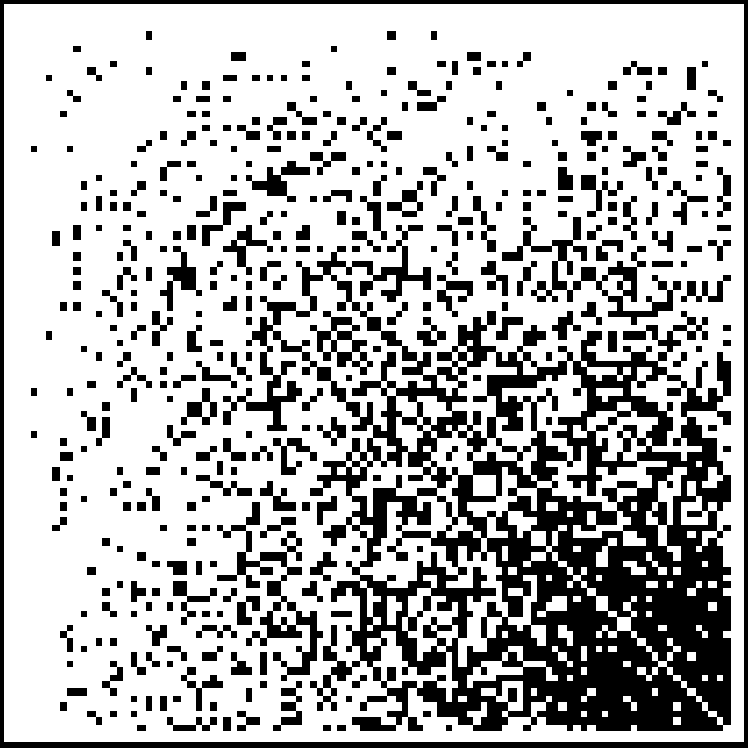
\includegraphics[width=0.18\columnwidth]{../figures/lovasz_sample100.pdf}
    %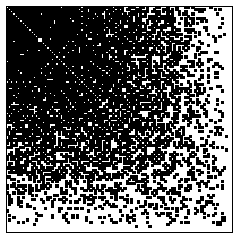
\includegraphics[width=2.8cm]{include/uniform_attachment_empirical.pdf}
  };
  \end{scope}
\end{tikzpicture}
